\section{Modules Description}
\subsection{Video Acquisition and Preprocessing}
\subsubsection{Frame Extraction and Normalization}
This module is responsible for converting raw video input into a structured and standardized format suitable for deep learning models. The system accepts an RGB video stream captured using a standard camera. Since deep learning models cannot directly operate on continuous video streams, the video is first decomposed into individual frames.

Frame extraction is performed using uniform sampling, where a fixed number of frames are selected from each video sequence. Uniform sampling preserves temporal information while avoiding redundant frames that do not contribute meaningful information. This step is especially important for real-time processing because it reduces computational overhead without losing critical motion cues.

Once extracted, each frame is resized to a predefined spatial resolution compatible with convolutional neural networks. Frame normalization is then applied by scaling pixel intensity values to a standard range. Normalization improves numerical stability during training and ensures consistent feature learning across videos captured under varying lighting conditions. Finally, all frame sequences are standardized to a fixed temporal length using padding or truncation, enabling efficient batch processing during training and inference.

\textbf{Output:} A fixed-length sequence of normalized RGB frames.

\subsubsection{Pose and Landmark Extraction}
This sub-module extracts structured motion and positional information from video frames. From each frame, key body, hand, and facial landmarks are detected to represent the signer's movements in a compact and meaningful form. These landmarks encode geometric relationships such as joint positions, hand orientation, and finger movement patterns.

Pose and landmark information provides complementary motion cues that are invariant to background noise and illumination changes. By representing gestures in terms of relative positions and movements, the system improves robustness to environmental variations. The extracted landmark features are temporally aligned with the corresponding RGB frames to preserve synchronization between visual appearance and motion information.

\textbf{Output:} A sequence of landmark feature vectors aligned with video frames.

The end-to-end preprocessing pipeline is shown in Fig.~\ref{fig:module-preprocess}.

\begin{figure}[H]
\centering
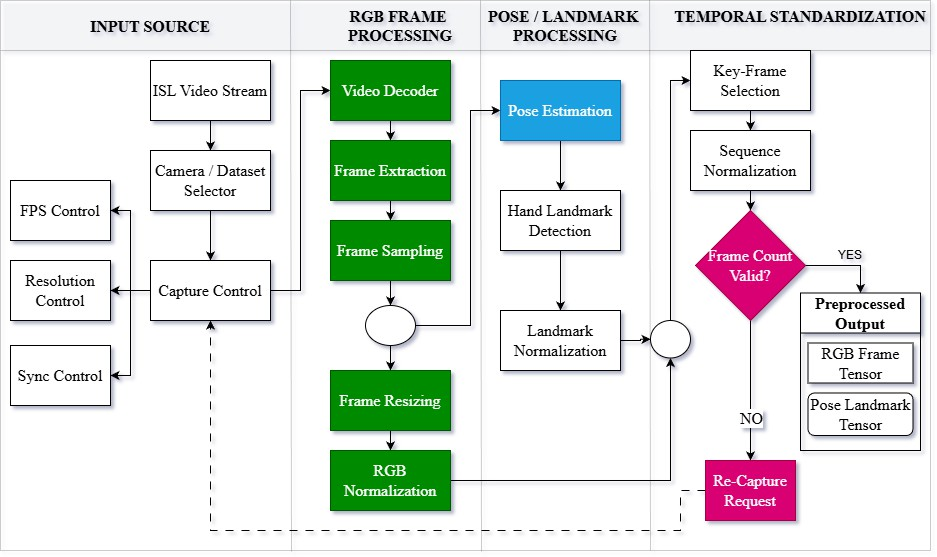
\includegraphics[width=\textwidth]{text/figures/docx_image2.jpeg}
\caption{Video Acquisition and Preprocessing Module.}
\label{fig:module-preprocess}
\end{figure}

\subsection{Feature Extraction and Fusion}
\subsubsection{RGB Feature Extraction Using CNN}
This module extracts spatial appearance features from RGB frames using a convolutional neural network (CNN). Each normalized frame is passed through multiple convolutional layers that learn hierarchical visual representations. Early layers capture low-level patterns such as edges and textures, while deeper layers learn high-level semantic features such as hand shape, orientation, and configuration.

The CNN transforms each frame into a compact feature vector that encodes visual characteristics relevant to sign language gestures. These features capture fine-grained appearance details that are critical for distinguishing visually similar signs.

\textbf{Output:} Frame-wise RGB feature vectors.

\subsubsection{Pose Feature Extraction and Attention-Based Fusion}
This sub-module processes the landmark feature vectors extracted in the preprocessing stage and integrates them with RGB features using an attention-based fusion mechanism. Pose features capture motion trajectories and relative positional changes, while RGB features provide detailed appearance information.

An attention mechanism is applied to dynamically assign importance weights to both RGB and pose features. During training, the model learns which feature type contributes more to recognizing a particular sign. For example, signs with subtle finger movements may rely more on landmark features, while signs with distinctive hand shapes may rely more on RGB features.

The attention-based fusion module suppresses irrelevant or noisy features and emphasizes discriminative information. The weighted RGB and pose features are then combined to form a unified spatiotemporal representation.

\textbf{Output:} Fused feature sequence containing both appearance and motion information.

The feature extraction and fusion stage is presented in Fig.~\ref{fig:module-fusion}.

\begin{figure}[H]
\centering
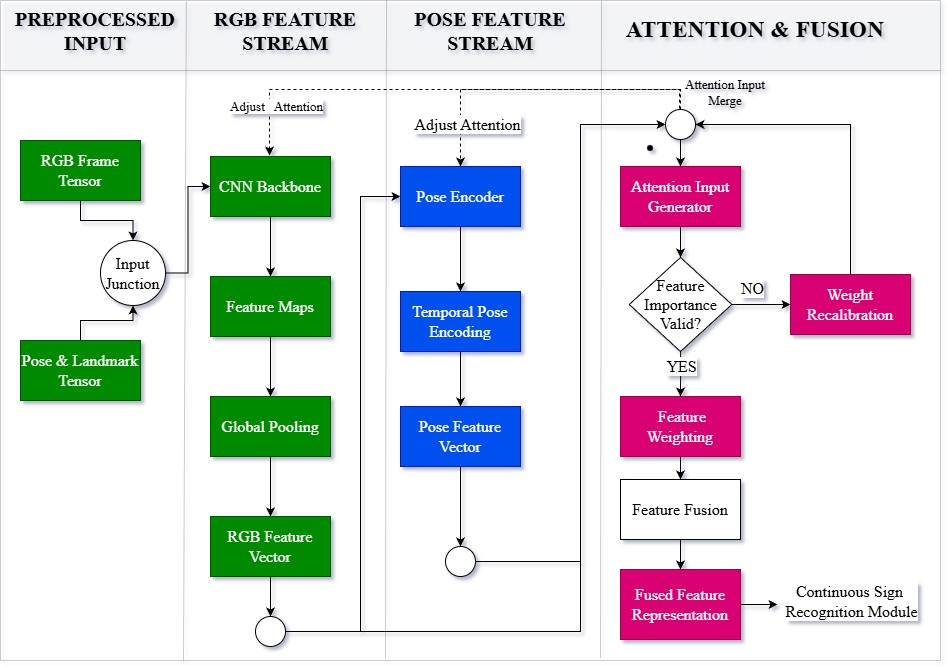
\includegraphics[width=\textwidth]{text/figures/docx_image3.jpeg}
\caption{Feature Extraction and Fusion Module.}
\label{fig:module-fusion}
\end{figure}

\subsection{Continuous Sign Recognition}
\subsubsection{Temporal Modeling Using Transformer or BiLSTM}
This module models the temporal evolution of the fused feature sequence. Since sign language gestures unfold over time, temporal modeling is essential for understanding gesture progression and context.

Two alternatives are considered:
\begin{itemize}[leftmargin=1.5em]
\item \textbf{BiLSTM:} processes the feature sequence in forward and backward directions to capture past and future dependencies.
\item \textbf{Transformer:} uses multi-head self-attention to model long-range dependencies across the sequence.
\end{itemize}

Temporal modeling enables the system to learn motion patterns, transitions between gesture components, and contextual relationships between frames. This is particularly important for continuous sign recognition, where multiple signs appear in a single video sequence.

\textbf{Output:} Context-aware temporal feature sequence.

\subsubsection{Sign Prediction Using CTC Decoder}
The temporally modeled feature sequence is passed to a Connectionist Temporal Classification (CTC) decoder. CTC enables sequence-to-sequence learning without requiring explicit alignment between frames and output labels.

During training, the CTC loss function allows the model to learn the most probable label sequence corresponding to the input feature sequence. During inference, a decoding strategy such as beam search is applied to generate the final predicted sign or sign sequence.

CTC is particularly effective for continuous sign recognition because it handles variable-length input and output sequences and naturally accounts for timing variations in gesture execution.

\textbf{Output:} Predicted sign or sign sequence.

The recognition module behavior is illustrated in Fig.~\ref{fig:module-recognition}.

\begin{figure}[H]
\centering
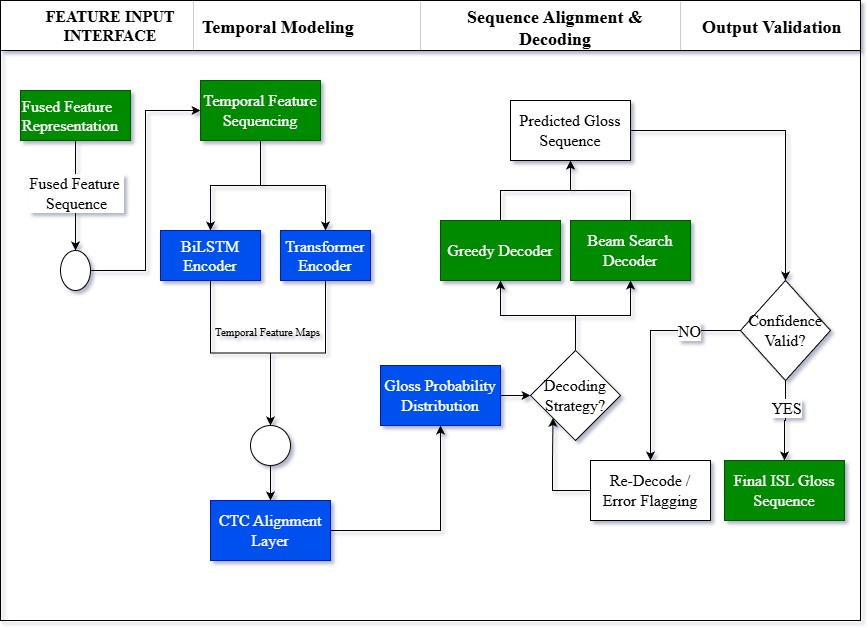
\includegraphics[width=\textwidth]{text/figures/docx_image4.jpeg}
\caption{Continuous Sign Recognition Module.}
\label{fig:module-recognition}
\end{figure}

\subsection{Language and Audio Output}
\subsubsection{Sentence Correction and Caption Buffer}
The predicted sign sequence is converted into textual form using a gloss-to-text mapping mechanism. Since the grammatical structure of sign language differs from spoken language, the generated text may contain syntactic inconsistencies.

A sentence correction module refines the generated text by correcting word order, grammatical errors, and incomplete phrases. A caption buffer is maintained to accumulate recognized signs over time, enabling smooth sentence formation in continuous recognition scenarios.

\textbf{Output:} Grammatically corrected text sentences.

The language and audio pipeline is shown in Fig.~\ref{fig:module-language-audio}.

\begin{figure}[H]
\centering
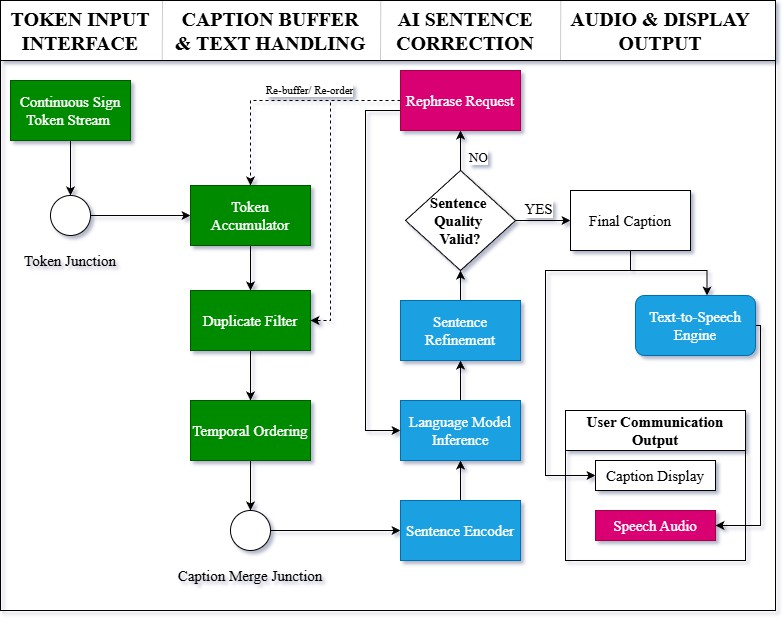
\includegraphics[width=\textwidth]{text/figures/docx_image5.jpeg}
\caption{Language and Audio Output Module.}
\label{fig:module-language-audio}
\end{figure}

\subsubsection{Text-to-Speech Output}
In the final module, corrected text is converted into audible speech using a text-to-speech engine. The TTS system generates natural-sounding audio corresponding to the recognized sign language content. This module enables real-time verbal communication between signing users and non-signing individuals.

\textbf{Output:} Spoken audio output.
